\chapter{KELP MODEL}
\label{chap:kelp}

In order to properly model the spatial distribution of light around the kelp, it is first necessary to formulate a spatial description of the kelp, which we do in this chapter.
We take a probabilistic approach to describing the kelp.
We begin by describing the distribution of kelp fronds, and through algebraic manipulation, we are able to assign to each point in space a probability that kelp occupies the location.


\section{Physical Setup}
The life of cultivated macroalgae generally begins in the laboratory, where microscopic kelp spores are inoculated onto a thread in a small laboratory pool.
This thread is wrapped around a larger rope as in Figure \ref{fig:rope_thread}, which is hung from buoys in the ocean.
The two primary configurations are vertical and horizontal or ``long'' lines.
In the case of vertical lines, the seaweed rope hangs straight down from a single buoy, and is either weighted or anchored.
In the case of long lines, the rope is strung from one buoy to another.
Long lines allow more light to reach the seaweed since it grows closer to the surface, but more vertical lines can be set up in a given area,
which may be advantageous for IMTA.

\begin{figure}[H]
  \centering
  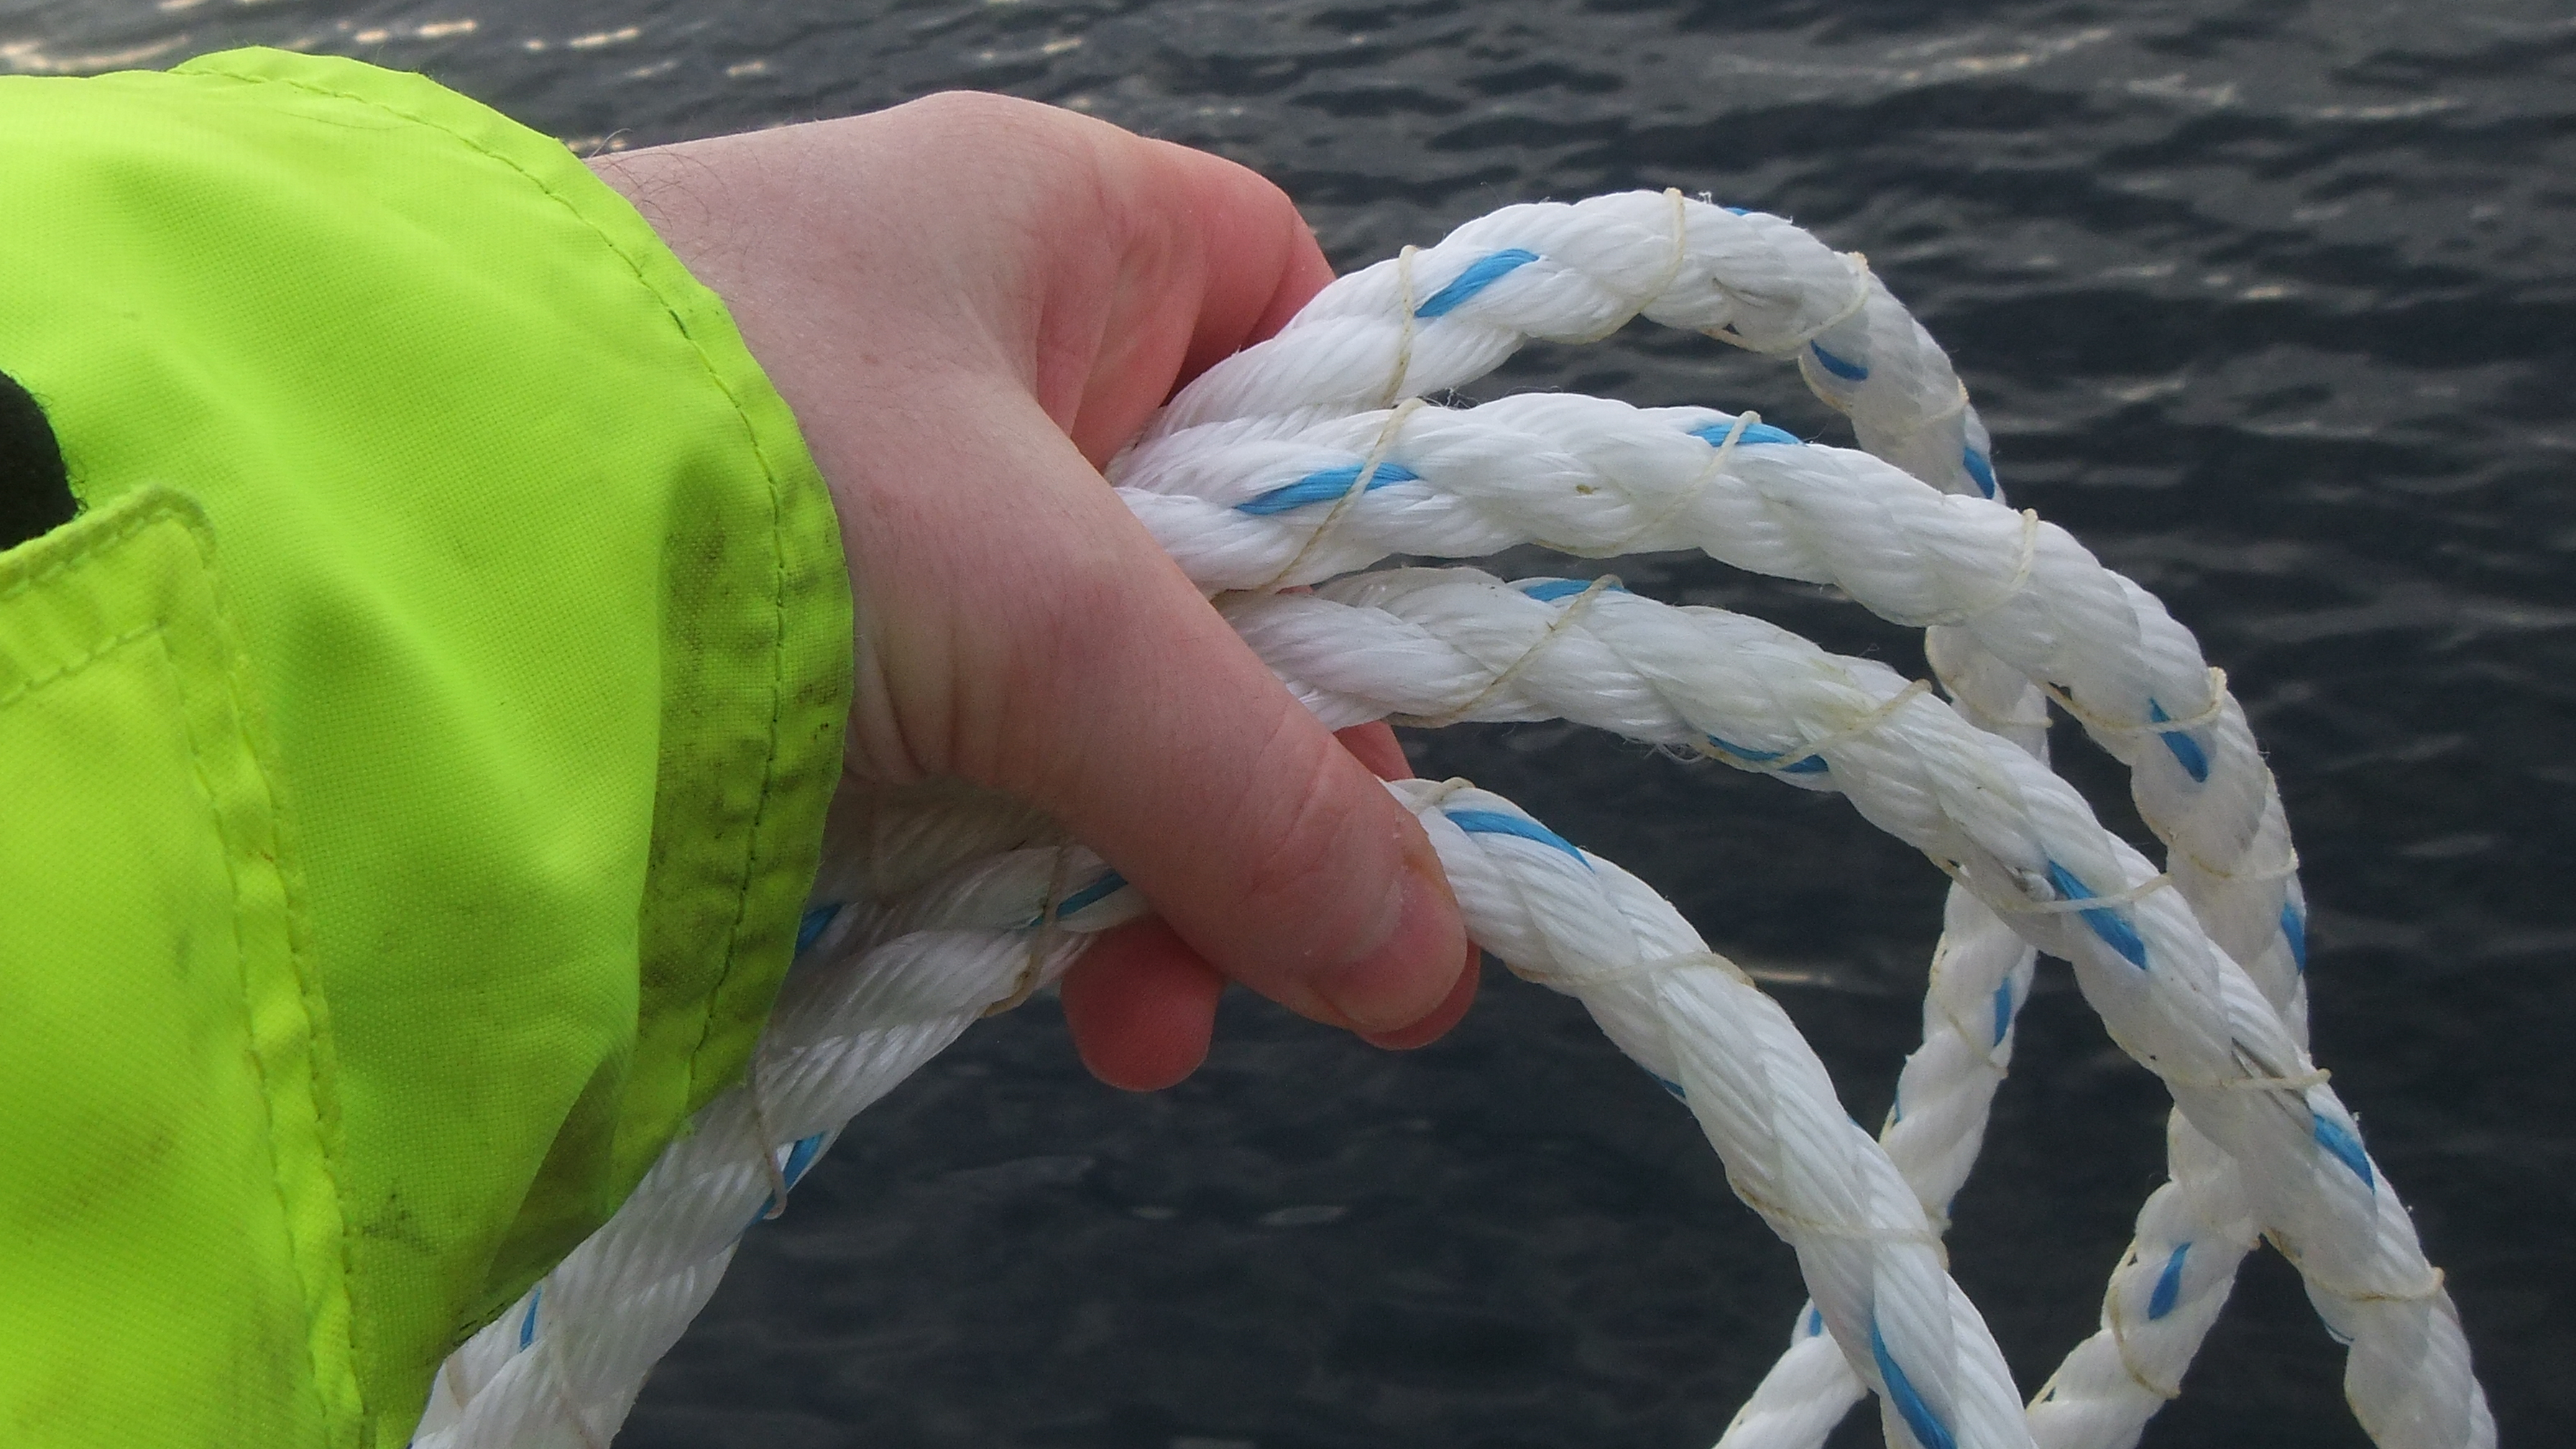
\includegraphics[width=0.65\textwidth]{kelp_photo/rope_thread}
  \caption{\textit{Saccharina latissima} innoculated onto a thread wrapped around a rope on which it is to be grown.}
  \label{fig:rope_thread}
\end{figure}

We consider only the case of a rigid vertical rope which does not sway in the current.
The mature \textit{Saccharina latissima} plant consists of a single frond (leaf), a stipe (stem) and a holdfast (root structure).
For the sake of this model, only the kelp frond is considered, and its base is attached directly to the rope.
The ``gentle undulation approximation'' is employed, whereby it is assumed that fronds are perfectly horizontal.
While at any given time they may point up or down due to water current and gravity, we consider the horizontal
state to be an average configuration.
This simplifaction allows for the three-dimensionally distributed population of kelp fronds
to be considered a collection of independent populations in two-dimensional depth layers.
A computer rendering of this scenario is shown in Figure \ref{fig:kelp_array}.

\begin{figure}[H]
	\centering
	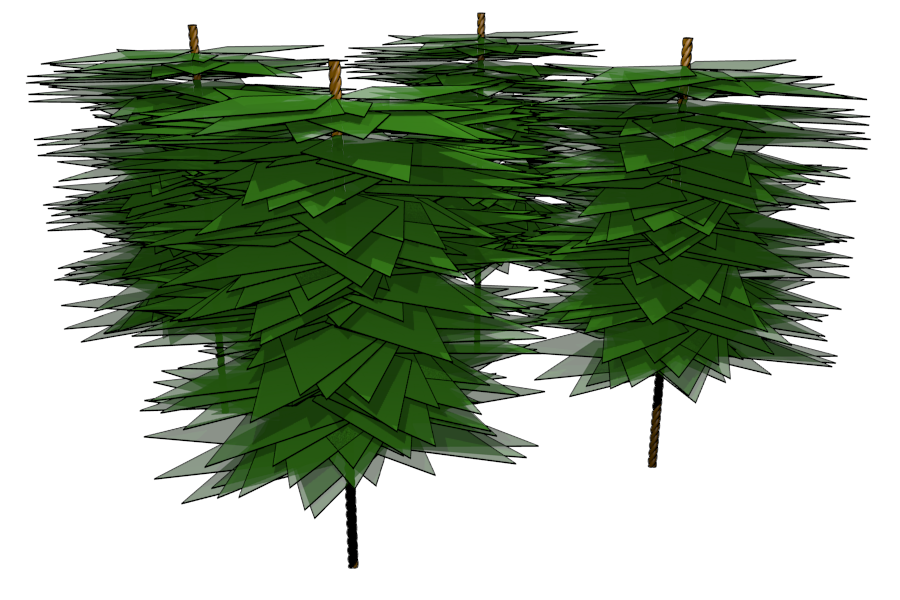
\includegraphics[width=3.5in]{kelp_array}
	\captionof{figure}{Rendering of four nearby vertical kelp ropes as represented in the spatial distribution model. Note the kite-shaped fronds and horizontal orientation.}
  \label{fig:kelp_array}
\end{figure}

\section{Coordinate System}
Consider the rectangular domain
\begin{align*}
  \xmin &\leq x \leq \xmax, \\
  \ymin &\leq y \leq \ymax, \\
  \zmin &\leq z \leq \zmax.
\end{align*}
For all three dimensional analysis, we use the absolute coordinate system defined in Figure \ref{fig:3dcoords}.
In the following sections, it is necessary to convert between Cartesian and spherical coordinates, which we do using the relations
\begin{equation}
  \left\{
	\begin{split}
		x & = r\sin\phi\cos\theta, \\
		y & = r\sin\phi\sin\theta, \\
		z & = r\cos\phi. \\
	\end{split}
  \right.
	\label{eqn:coords}
\end{equation}
Therefore, for some function $f(x,y,z)$, we can write its derivative along a path in spherical coordinates in terms of Cartesian coordinates using the chain rule,
\begin{equation*}
	\frac{\partial f}{\partial r}
	=\frac{\partial f}{\partial x}\frac{\partial x}{\partial r}
	+ \frac{\partial f}{\partial y}\frac{\partial y}{\partial r}
	+ \frac{\partial f}{\partial z}\frac{\partial z}{\partial r}.
\end{equation*}
Then, calculating derivatives from \eqref{eqn:coords} yields
\begin{equation}
	\frac{\partial f}{\partial r}
	=\frac{\partial f}{\partial x}\sin\phi\cos\theta
	+ \frac{\partial f}{\partial y}\sin\phi\sin\theta
	+ \frac{\partial f}{\partial z}\cos\phi.
	\label{eqn:partials}
\end{equation}
\begin{figure}[H]
	\centering
	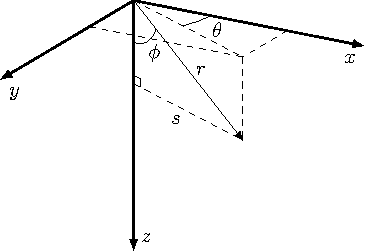
\includegraphics[width=3in]{3d_coords}
	\caption{Downward-facing right-handed coordinate system with radial distance $r$ from the origin, distance $s$ from the $z$ axis, zenith angle $\phi$ and azimuthal angle $\theta$.}
	\label{fig:3dcoords}
\end{figure}

\section{Population Distributions}
In order to construct a spatial distribution of kelp fronds, a simple kite-shaped geometry is introduced,
and frond lengths and azimuthal orientations are assumed to be distributed predictably.
Since it is assumed that fronds extend perfectly horizontally, no angular elevation distribution is required.

\subsection{Frond Shape}
\label{sec:shape}

\begin{figure}[h]
	\centering
  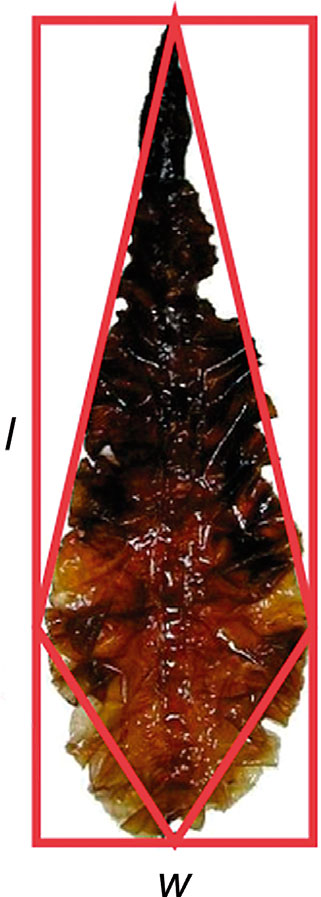
\includegraphics[width=1.2in]{kelp_photo/kite}
  %TODO: Cite this?
  \qquad
	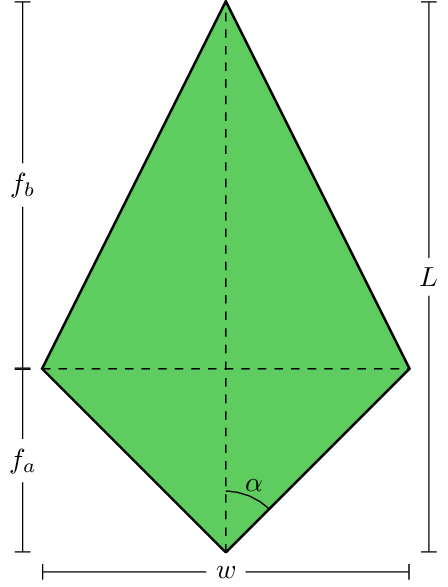
\includegraphics[width=2in]{frond}
	\captionof{figure}{Simplified kite-shaped frond.}
	\label{fig:frond}
\end{figure}

The frond is assumed to be kite-shaped with length $l$ from base to tip, and width $w$ from left to right.
In Figure \ref{fig:frond}, the base is shown at the bottom and the tip is shown at the top.
The proximal length is the shortest distance from the base to the diagonal connecting the left and right corners, and is notated as $f_a$.
Likewise, the distal length is the shortest distance from that diagonal to the tip, notated $f_b$.
It is therefore clear that
 \begin{equation*}
	 f_a + f_b = l.
 \end{equation*}
When considering a whole population with varying sizes, it is more convenient to specify ratios than absolute lengths.
Define the ratios
\begin{align*}
	f_r &= \frac{l}{w}, \\
	f_s &= \frac{f_a}{f_b}.
\end{align*}
These ratios are assumed to be constant among the entire population, so that all fronds are geometrically similar.
Thus, the shape of the frond can be fully specified by $l$, $f_r$, and $f_s$;
it is possible to redefine $w$, $f_a$ and $f_b$ from the preceding formulas as
\begin{align*}
	w &= \frac{l}{f_r}, \\
	f_a &= \frac{lf_s}{1+f_s}, \\
	f_b &= \frac{l}{1+f_s}.
\end{align*}
The angle $\alpha$, half of the angle at the base corner, is also noteworthy.
From the above equations, it follows that
\begin{equation*}
	\alpha = \tan^{-1}\left(\frac{2f_rf_s}{1+f_s}\right).
\end{equation*}

It is useful to convert between frond length and surface area, which can be done via the relations
\begin{align}
  A &= \frac{lw}{2} = \frac{l^2}{2f_r}, \\
  l &= \sqrt{2Af_r}.
  \label{eqn:length-from-area}
\end{align}

\subsection{Length and Angle Distributions}
\label{sec:dist}
The distribution of frond lengths is assumed to be normal, with mean $\mu_l$ and standard deviation $\sigma_l$.
That is, it has the probability density function (PDF)
\begin{equation*}
  P_l(l) = \frac{1}{\sqrt{2\pi\sigma_l^2}}\exp\left(\frac{(l-\mu_l)^2}{2\sigma_l^2}\right).
\end{equation*}

It is further assumed that frond angle varies according to the von Mises distribution, which is the periodic analogue of the normal distribution, defined on $[-\pi,\pi]$ rather than $(-\infty,\infty)$.
The von Mises distribution has two parameters, $\mu$ and $\kappa$, which shift and sharpen its peak respectively, as shown in Figure \ref{fig:vonmises}.
$\kappa$ is analogous to $1/\sigma$ in the normal distribution.
In the absence of current, the frond angles are be distributed uniformly, while as current velocity increases, they become increasingly likely to align in the current direction, depending on the stiffness of the frond.
Assuming a linear relationship between the current velocity and the steepness of the angular distribution, define the \textit{frond alignment coefficient} $\eta$, with units of inverse velocity(\SI{}{\s\per\m}).
Then, use $\mu = \theta_w$ and $\kappa = \eta v_w$ as the von Mises distribution parameters.
Note that $\theta_w$ and $v_w$ vary over depth, while $\eta$ is assumed constant for the population.
Then, the PDF for the von Mises frond angle distribution is
\begin{equation*}
	P_{\theta_f}(\theta_f) = \frac{\exp\left(\eta v_w\cos(\theta_f-\theta_w)\right)}{2\pi I_0(\eta v_w)},
\end{equation*}
where $I_0(x)$ is the modified Bessel function of the first kind of order 0.
Notice that unlike the normal distribution, the von Mises distribution approaches a \textit{non-zero} uniform distribution as $\kappa$ approaches 0, so
\begin{equation*}
	\displaystyle \lim_{v_w \to 0}P_{\theta_f}(\theta_f) = \frac{1}{2\pi} \;\forall\, \theta_f \in [-\pi,\pi].
\end{equation*}

\begin{figure}[h]
	\centering
	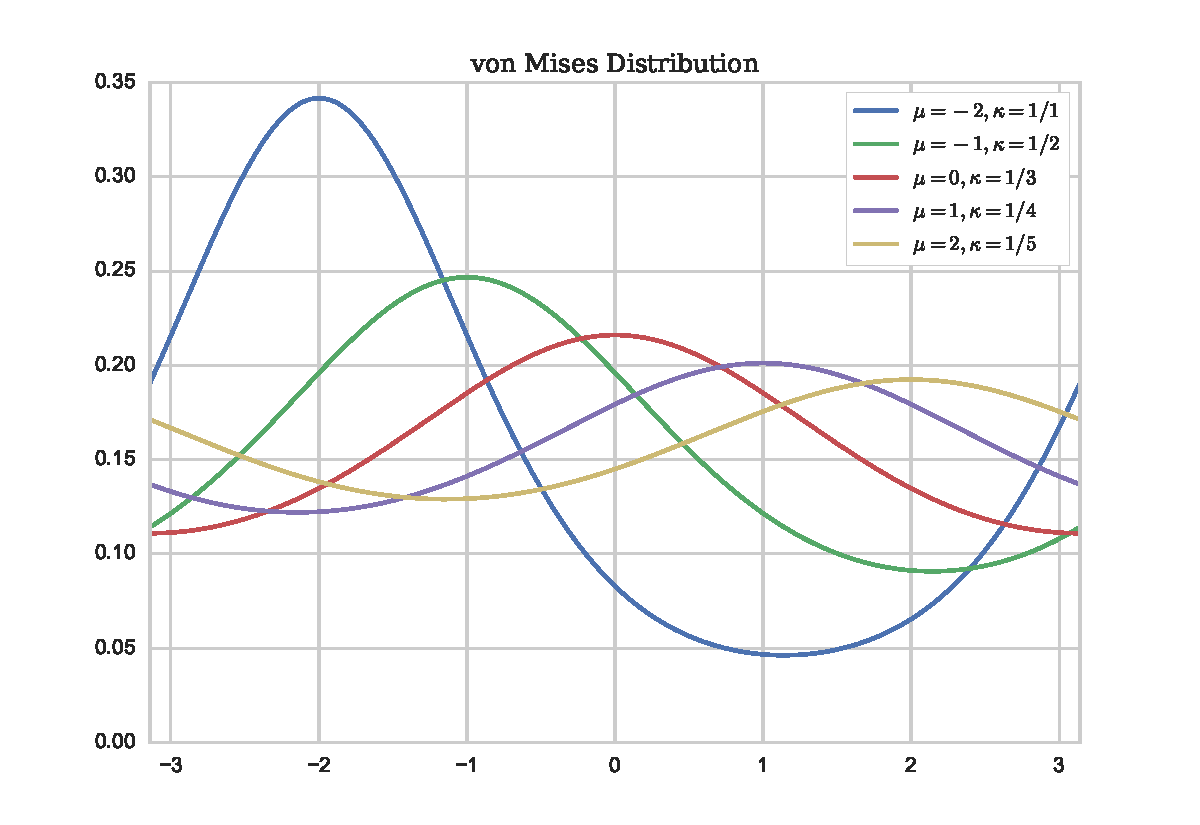
\includegraphics[width=6in]{vonmises}
	\captionof{figure}{von Mises distribution for a variety of parameters.}
	\label{fig:vonmises}
\end{figure}

\subsection{Joint Length-Orientation Distribution}
\label{sec:dist_2d}
The previous two distributions can reasonably be assumed to be independent of one another. That is, the angle of the frond does not depend on the length, or vice versa.
Therefore, the probability of a frond simultaneously having a given frond length and angle is the product of their individual probabilities.
Given independent events $A$ and $B$, the probability of their intersection is the product of their individual probabilities.
That is,
\begin{equation*}
	\label{eq:ind_prob}
	P(A \cap B) = P(A)P(B).
\end{equation*}
Then the probability of frond length $l$ and frond angle $\theta_f$ coinciding is
\begin{equation*}
	P_{2D}(\theta_f,l) = P_{\theta_f}(\theta_f) \cdot P_l(l).
\end{equation*}
A contour plot of this 2D distribution for a specific set of parameters is shown in Figure \ref{fig:dist_2d}, where probability is represented by color in the 2D plane.
Darker green represents higher probability, while lighter beige represents lower probability.
In Figure \ref{fig:kelp_sample}, 50 samples are drawn from this distribution and plotted.

It is important to note that if $P_{\theta_f}$ were dependent on $l$, the above definition of $P_{2D}$ would no longer be valid.
For example, it might be more realistic to say that larger fronds are less likely to bend towards the direction of the current.
In this case, \eqref{eq:ind_prob} would no longer hold, and it would be necessary to use the more general relation
\begin{equation*}
	P(A \cap B) = P(A)P(B|A) = P(B)P(B|A),
\end{equation*}
which is currently not taken into consideration in this model.

\begin{figure}[h]
	\centering
	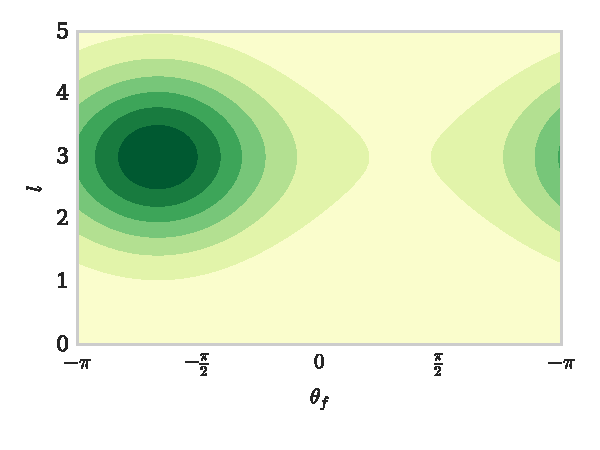
\includegraphics[width=4.5in]{prob_2d}
	\captionof{figure}{2D length-angle probability distribution with $\theta_w=7\pi/4$, $v_w=1$, $\mu_l=3$, $\sigma_l=1$.}
	\label{fig:dist_2d}
\end{figure}

\begin{figure}[h]
	\centering
	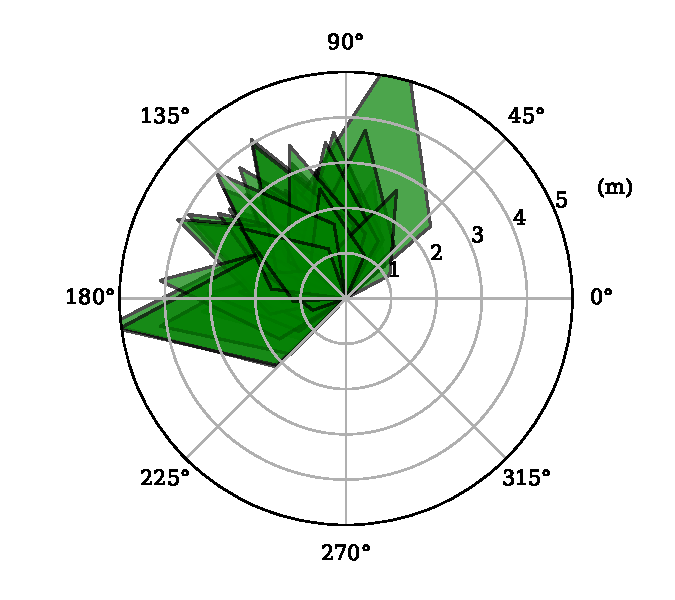
\includegraphics[width=4.5in]{kelp_sample}
	\captionof{figure}{A sample of 50 kelp fronds with shape parameters $f_s=0.5$ and $f_r=2$ whose lengths are picked from a normal distribution and whose angles are picked from a von Mises distribution.}
	\label{fig:kelp_sample}
\end{figure}

\section{Spatial Distribution}
In this section, the population length and angle distributions from the previous section are used to construct a spatial distribution of kelp.
This is made possible by the simple kite-shape fronds, and would be considerably more difficult with more general frond shapes.
\subsection{Rotated Coordinate System}
\label{sec:rot_coords}
To determine under what conditions a frond will occupy a given point, we begin by
describing the shape of the frond in Cartesian coordinates and then convert to polar coordinates.
Of primary interest are the edges connected to the frond tip.
For convenience, we will use a rotated coordinate system $(\theta',s)$ such that the line connecting the base to the tip is vertical, with the base at $(0,0)$.
Denote the Cartesian analogue of this coordinate system as $(x',y')$ which is related to $(\theta',s)$ by
\begin{align*}
	x' &= s\cos\theta' \\
	y' &= s\sin\theta' \\
	s &= \sqrt{x'^2+y'^2}, \\
	\theta' &= \atantwo(y, x).
\end{align*}

\subsection{Functional Description of Frond Edge}
With this coordinate system established, the outer two edges of the frond can be described in Cartesian coordinates as a piecewise linear function connecting the left corner: $(-w/2,f_a)$, the tip: $(0,l)$, and the right corner: $(w/2,f_a)$.
This function has the form
\begin{equation*}
	y'_f(x') = l-\sign(x')\frac{f_b}{w/2}x'.
\end{equation*}
Using the equations in Section \ref{sec:rot_coords}, this can be written in polar coordinates after some rearrangement as
\begin{equation*}
	s_f'(\theta') = \frac{l}{\sin\theta' + S(\theta')\frac{2f_b}{w}\cos\theta'},
\end{equation*}
where
\begin{equation*}
	S(\theta') = \sign(\theta'-\pi/2).
\end{equation*}
Then, using the relationships in Section \ref{sec:shape}, the above equation can be rewritten in terms of the frond ratios $f_s$ and $f_r$ as
\begin{equation*}
	\label{eq:rf_rel}
	s_f'(\theta') = \frac{l}{\sin\theta' + S(\theta')\frac{2f_r}{1+f_s}\cos\theta'}.
\end{equation*}
To generalize to a frond pointed at an angle $\theta_f$, we introduce the coordinate system $(\theta,s)$ such that
\begin{equation*}
	\theta = \theta' + \theta_f - \frac{\pi}{2}.
\end{equation*}
Then, for a frond pointed at the arbitrary angle $\theta_f$, the function for the outer edges can be written as
\begin{equation*}
	\label{eq:rf_abs}
	s_f(\theta) = s_f'\left(\theta - \theta_f + \frac{\pi}{2} \right).
\end{equation*}

\subsection{Conditions for Occupancy}
We now formulate the conditions under which a kite shape frond occupies a point
in the sense that the point lies within its interior.
Combining these conditions with the size and orientation distributions from \ref{sec:dist}
allows a spatial distribution of the kelp fronds to be calculated.

Consider a fixed frond of length $l$ at an angle $\theta_f$. The point
$(\theta,s)$ is occupied by the frond if
\begin{align*}
	\left|\theta_f - \theta \right| < \alpha,
	s < s_f(\theta).
\end{align*}

Equivalently, the opposite perspective can be taken.
Letting the point $(\theta,s)$ be fixed, a frond occupies the point if
\begin{align}
	\theta - \alpha < \theta_f < \theta + \alpha,
	\label{eqn:rs_th} \\
	l > l_{min}(\theta,s),
	\label{eqn:rs_l}
\end{align}
where
\begin{equation*}
	l_{min}(\theta,s) = s \cdot \frac{l}{s_f(\theta)}.
\end{equation*}
Then, considering the point to be fixed, \eqref{eqn:rs_th} and \eqref{eqn:rs_l} define the spacial region $R_s(\theta,s)$ called the ``occupancy region for $(\theta,s)$'' with the property that if the tip of a frond lies within this region (i.e., $(\theta_f,l) \in R_s(\theta,s)$), then it occupies the point.
$R_s(3\pi/4,1.5)$ is shown in blue in Figure \ref{fig:shade_area} and the smallest possible occupying fronds for several values of $\theta_f$ are shown in various colors.
Any frond longer than these at the same angle will also occupy the point.

\begin{figure}[h]
	\centering
	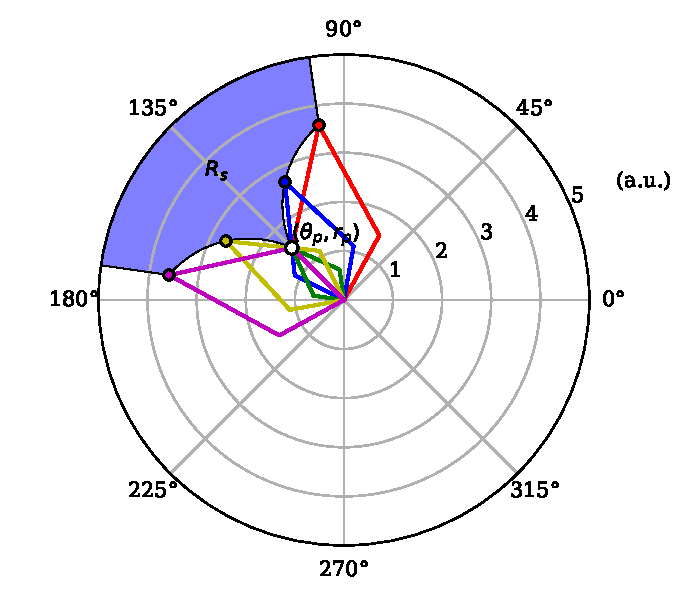
\includegraphics[width=4.5in]{shade_area}
	\captionof{figure}{Outlines of minimum-length fronds for a variety of angles to occupy the point $(\theta,s)=(3\pi/4,3/2)$.}
	\label{fig:shade_area}
\end{figure}

\subsection{Probability of Occupancy}
We are interested in the probability that, given a fixed point $(\theta,s)$, values of $l$ and $\theta_f$ chosen from the distributions described in Section \ref{sec:dist} will fall in the occupancy region.
This is found by integrating $P_{2D}$ over the occupancy region for $(\theta,s)$.

\begin{figure}[h]
	\centering
	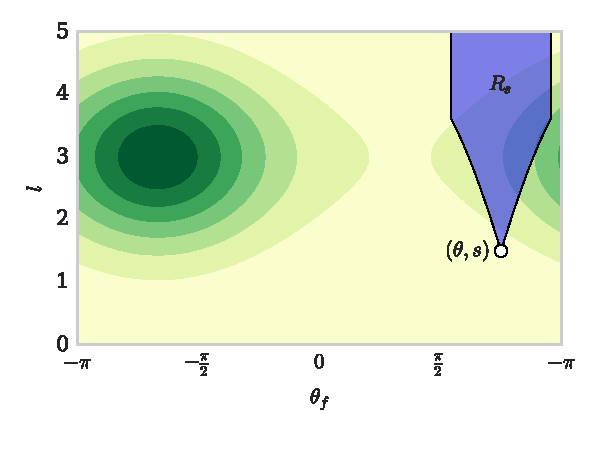
\includegraphics[width=4.5in]{cart_shade}
	\captionof{figure}{Contour plot of $P_{2D}(\theta_f,l)$ overlayed with the
    region in the $\theta_f$\nobreak-\nobreak$l$ plane which results in a frond occupying the point $(\theta,s)=(3\pi/4,3/2)$.}
	\label{fig:cart_shade}
\end{figure}

Integrating $P_{2D}(\theta_f,l)$ over $R_s(\theta,s)$ as depicted in Figure \ref{fig:cart_shade} yields the proportion of the population in the depth layer occupying the point $(\theta,s)$,
\begin{align*}
		\tilde{P}_k(\theta,s,z)	&= \iint_{R_s(\theta,s)}
								P_{2D}(\theta_f,l)
								\,dl\,d\theta_f \nonumber \\
							&= \int_{\theta-\alpha}^{\theta+\alpha}
								\int_{l_{min}(\theta_f)}^\infty
								P_{2D}(\theta_f,l)
								\,dl\,d\theta_f.
\end{align*}

Assuming that the depth layer has thickness $dz$ and contains $n$ fronds of thickenss $t$,
the proportion of the depth layer occupied by kelp at any horizontal position can be calculated as
\begin{equation*}
  P_k = \frac{nt}{dz}\tilde{P}_k.
\end{equation*}
Then, the effective absorption coefficient can be calculated at any point in space as
\begin{equation*}
  a(\vec{x}) = P_k(\vec{x})a_k + (1-P_k(\vec{x}))a_w.
\end{equation*}

\begin{figure}[h]
	\centering
	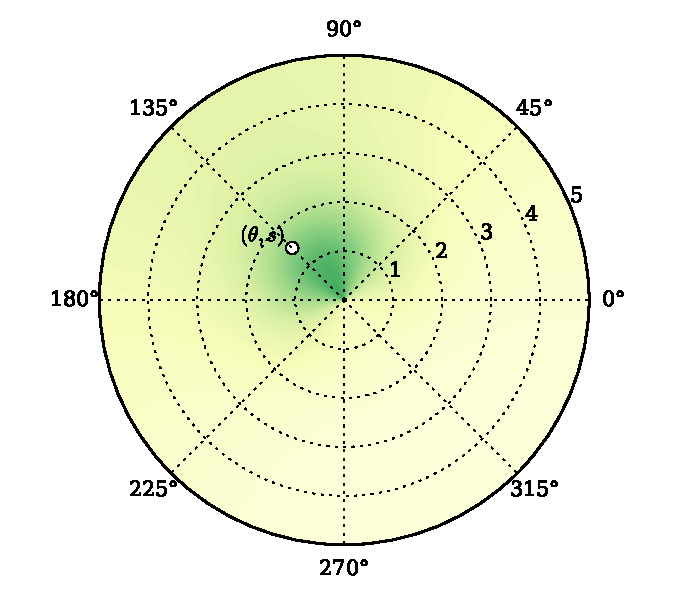
\includegraphics[width=4.5in]{prob_shade}
	\captionof{figure}{Contour plot of the probability of frond occupation sampled at 121 points using $\theta_f=2\pi/3,\eta v_w=1$.}
	\label{fig:prob_shade}
\end{figure}
